% ch01b: 印刷页 9--14（§1.2 末 + §1.3）
现在回忆 $G$ 的辛叶（symplectic leaf）分类（例如见 [12, 19]）。群 $G$ 可以分解为双 Bruhat 胞腔之并
\[
G=\bigsqcup_{u\in W\times W}G_u,
\]
指标取遍群 $W\times W$ 的元素，其中 $W$ 是 $G$ 的外尔群。每个双 Bruhat 胞腔都是同型的，即它双有理等价于一个辛流形与一个 Poisson 括号平凡的流形的乘积。胞腔 $G_u$ 的维数由
\[
\dim G_u=l(u)+\operatorname{rank}G
\]
给出，其中 $l(u)$ 是 $u$ 的长度。

可以对 Poisson 流形 $G$ 略作修改，使所有构造都更对称一些。具体地说，考虑嘉当（Cartan）子群 $H\subset G$ 在 $G$ 上以共轭作用。由于 $H$ 是 $G$ 的 Poisson 子群、其 Poisson 结构平凡，商 $G/\operatorname{Ad}H$ 继承 Poisson 结构、Poisson 交换函数族 $\{\mathcal H_i\}$，以及分解为 Poisson 子流形
\[
G/\operatorname{Ad}H=\bigsqcup_{u\in W\times W}G_u/\operatorname{Ad}H.
\]
相应 Poisson 子流形的维数现在恰好是 $\dim G_u/\operatorname{Ad}H=l(u)$。

\section{双 Bruhat 胞腔的簇参数化：单群}

沿用 [4]，我们在本节描述如何在 $G_u$ 与 $G_u/\operatorname{Ad}H$ 上引入簇代数簇的结构。具体地说，从 $u$ 作为 $W\times W$ 的标准生成元的约化乘积的分解 $u=s_{i_1}\cdots s_{i_l}$ 出发，我们定义一个簇种子（见附录 1.9）——一个带对数常值 Poisson 结构的可裂代数环面——以及它到 $G_u$ 的 Poisson 嵌入，其像为 Zariski 开集。类似地，由同一组数据可以构造 $G_u/\operatorname{Ad}H$ 的簇种子。最后我们证明：当 $G=\operatorname{PGL}(N)$ 时，这些簇种子同构于由圆盘上由分解 $u=s_{i_1}\cdots s_{i_l}$ 所构造的 Thurston 图对应的簇种子。

\subsection{单群的 Cartan--Weyl 生成元}

为描述 $G_u$ 与 $G_u/\operatorname{Ad}H$ 上的簇坐标，我们首先需要引入李群 $G$ 的一组生成元，它们与相应李代数 $\mathfrak g$ 的 Cartan--Weyl 生成元类似。外尔群 $W$ 的标准生成元集合与 $G$ 的单根集合 $\Pi$ 有典范双射，我们不再区分这两个集合。第二份 $W$ 的生成元集合则与负单根集合 $\overline\Pi$ 等同。

回忆：给定嘉当矩阵 $C_{ij}$，相应的李代数 $\mathfrak g$ 由 $\{h_i\mid i\in\Pi\}$ 与 $\{e_i\mid i\in\Pi\cup\overline\Pi\}$ 生成，并满足下列关系（为简单起见，记 $\bar\imath$ 为与根 $i$ 相反的根，并把 $h$ 与 $C$ 延拓到负根，约定 $h_i=h_{\bar\imath}$、$C_{\bar\imath,\bar\jmath}=C_{ij}$，且当 $i$ 与 $j$ 符号不同时 $C_{ij}=0$）：
\begin{equation}\label{eq:1.3}
\begin{aligned}
&[h_i,h_j]=0,\\
&[h_i,e_j]=\operatorname{sign}(j)C_{ij}e_j,\\
&[e_i,e_{\bar\imath}]=\operatorname{sign}(i)h_i,\\
&(\operatorname{ad}e_i)^{1-C_{ij}}e_j=0\quad\text{对 } i+j\neq0.
\end{aligned}
\tag{1.3}
\end{equation}

对同一李代数，可以把集合 $\{h_i\}$ 换为由
\[
h_i=\sum_{j\in\Pi}C_{ij}h^j
\]
定义的集合 $\{h^i\}$，此时关系 (1.3) 取下述形式：
\begin{equation}\label{eq:1.4}
\begin{aligned}
&[h^i,h^j]=0,\\
&[h^i,e_j]=\operatorname{sign}(j)\delta^i_j\,e_j,\\
&[e_i,e_{\bar\imath}]=\operatorname{sign}(i)C_{ij}h^j,\\
&(\operatorname{ad}e_i)^{1-C_{ij}}e_j=0\quad\text{对 } i+j\neq0.
\end{aligned}
\tag{1.4}
\end{equation}

对任意 $i\in\Pi\cup\overline\Pi$ 引入群元素 $E_i=\exp(e_i)$ 与单参数子群 $H_i(x)=\exp(h^i\log x)$，它们将作为群 $G$ 的生成元组。交换关系 (1.4) 蕴涵 $H_i$ 与 $E_i$ 之间的关系（对单链情形，我们在附录 1.10 中列出）。由 (1.4) 立即可见：只要 $i\neq j$，$H_i(x)$ 就与 $E_j$ 交换；又若 $C_{ij}=0$ 且 $i\neq\bar\jmath$，则 $E_i$ 与 $E_j$ 交换。

\subsection{簇种子的构造}

取元素 $u\in W\times W$ 的一个分解 $u=s_{i_1}\cdots s_{i_l}$。与这样的 $u$ 相联系的有簇种子 $((\C^\times)^l,\varepsilon)$ 以及映射 $\mathrm{ev}\colon(\C^\times)^l\to G/\operatorname{Ad}H$：
\begin{equation}\label{eq:1.5}
(x_1,\dots,x_l)\mapsto H_{i_1}(x_1)E_{i_1}\cdots H_{i_l}(x_l)E_{i_l}.
\tag{1.5}
\end{equation}
该映射的像在双 Bruhat 胞腔 $G_u$ 中是 Zariski 开的；当词 $u$ 约化时，它是嵌入。同一元素 $u\in W\times W$ 的不同约化分解给出不同的参数化，它们之间由簇变换相联系。

要构造簇种子 $((\C^\times)^{l+r},\varepsilon)$（其中 $r$ 是 $G$ 的秩），即参数化单群 $G$ 自身的胞腔，只需把上述表达式从右乘以嘉当子群的任意元素：
\begin{equation}\label{eq:1.6}
(x_1,\dots,x_{l+r})\mapsto H_{i_1}(x_1)E_{i_1}\cdots H_{i_l}(x_l)E_{i_l}H_1(x_{l+1})\cdots H_r(x_{l+r}).
\tag{1.6}
\end{equation}
相应的交换矩阵 $\varepsilon$ 的构造见附录 1.11。

利用除非 $i=j$ 否则 $H_i(x)E_j=E_jH_i(x)$ 这一事实，可以通过把任意 $H_i$ 一直移动到它遇到 $E_i$ 或 $E_{\bar\imath}$ 为止，把表达式 (1.5) 与 (1.6) 改写成许多不同的形式。因此，每个簇变量自然地联系到一个正单根 $i$；并且对给定的 $i$，联系到词 $s_{i_1}\cdots s_{i_l}$ 的一个极小线段，该线段由 $s_i$、$s_{\bar\imath}$ 或词的端点所界定（对循环词，所有线段都只由 $s_i$ 或 $s_{\bar\imath}$ 界定）。

可以验证（见 [4]）：同一词 $u$ 的不同分解所对应的簇种子由簇变换相联系。特别地，它们的像在余维一的意义下重合。例如若 $C_{ij}=C_{ji}=-1$，则对应于分解 $u=As_is_js_iB$（其中 $A,B$ 是任意词）的坐标，与对应于分解 $\tilde u=As_js_is_jB$ 的坐标，由一个关于线段 $[s_is_js_i]$ 的簇变量的变异相联系。类似地，$As_is_{\bar\imath}B$ 与 $As_{\bar\imath}s_iB$ 之间的关系是作一个关于线段 $[s_is_{\bar\imath}]$ 的变异。若 $C_{ij}=0$，则应用关系 $As_is_jB\leftrightarrow As_js_iB$ 不改变参数化，因为相应的矩阵 $E_i$ 与 $E_j$ 交换。

若分解不是约化的，映射 (1.5) 与 (1.6) 仍有定义，但不再是嵌入。此时它们等于某个约化词所对应的嵌入，复合上沿某些坐标的投影以及若干变异。事实上，词 $As_is_iB$ 对应的映射，是关于线段 $[s_is_i]$ 的变异与 $As_iB$ 对应的映射的复合。

因此我们断言：$G$ 与 $G/\operatorname{Ad}H$ 的双 Bruhat 胞腔都是簇代数簇。在 [4] 中证明了：由交换矩阵 $\varepsilon$ 给出的 $G_u$（从而 $G_u/\operatorname{Ad}H$）上的 Poisson 括号，与由 Drinfeld--Jimbo $r$-矩阵 (1.2) 给出的 Poisson 括号确实相同。

\subsection{群 PGL(N) 的生成元与 Thurston 图}

当 $G=\operatorname{PGL}(N)$ 时，该构造可以写得具体得多。$E_i$ 与 $H_i(x)$ 在标准表示中具有特别简单的形式：
\begin{equation}\label{eq:1.7}
H_i(x)=
\begin{pmatrix}
x&0&\cdots&&0\\
0&\ddots&&&&\\
\vdots&&x&&&\\
&&&1&\ddots&\\
&&&&\ddots&0\\
0&&&&&1
\end{pmatrix},
\qquad
E_i=E_{\bar\imath}^{\mathrm{tr}}=
\begin{pmatrix}
1&0&\cdots&&0\\
0&\ddots&&&&\\
\vdots&&1&1&&\\
&&&&\ddots&0\\
0&&&&&1
\end{pmatrix},
\tag{1.7}
\end{equation}
其中 $H_i(x)$ 中含 $x$ 的最下面一行、以及 $E_i$ 中含非对角 $1$ 的那一行，其行号为 $i>0$。对负的 $i$，相应的矩阵 $E_{-i}=E_{\bar\imath}$ 只需取正根对应矩阵的转置。

现在用 Thurston 图给出另一种描述：把 $u\in W\times W$ 分解为 $\operatorname{PGL}(N)$ 的生成元之乘积（见附录 1.12）。$u$ 的每个分解为生成元之乘积都对应于一个 Thurston 图，后者又对应于一个簇种子。我们断言，这种替代方式给出同一个种子。为验证此断言，首先需要比较对应于单个生成元的种子：这可以通过比较只含一个三重点的初等 Thurston 图的交换图（见图 1.1 A）与附录 1.11 所描述的交换图（弦）来完成。其次需要验证：粘合交换图对应于粘合 Thurston 图。这些验证留作容易的练习。

\begin{figure}[htbp]
\centering
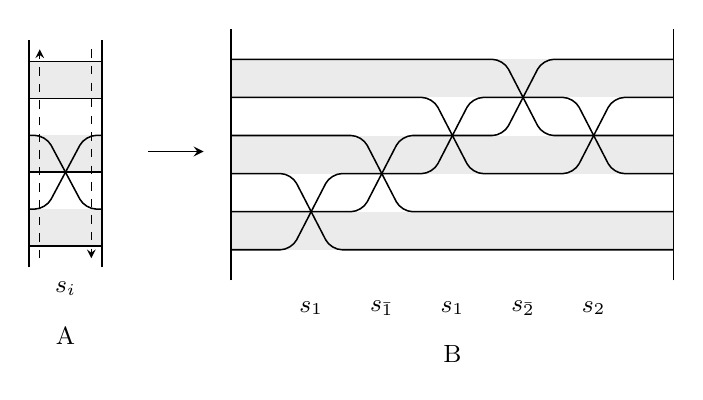
\begin{tikzpicture}[scale=0.78]
\begin{scope}[yshift=0.35]
\fill[black!8] (0,0.40) rectangle (1.20,1.00);
\fill[black!8] (0,1.60) rectangle (1.20,2.20);
\fill[black!8] (0,2.80) rectangle (1.20,3.40);
\draw[line width=0.55pt,rounded corners=4pt] (0,0.40) -- (1.20,0.40);
\draw[line width=0.55pt,rounded corners=4pt] (0,1.00) -- (0.28,1.00) -- (0.60,1.60) -- (0.92,2.20) -- (1.20,2.20);
\draw[line width=0.55pt,rounded corners=4pt] (0,1.60) -- (1.20,1.60);
\draw[line width=0.55pt,rounded corners=4pt] (0,2.20) -- (0.28,2.20) -- (0.60,1.60) -- (0.92,1.00) -- (1.20,1.00);
\draw[line width=0.55pt,rounded corners=4pt] (0,2.80) -- (1.20,2.80);
\draw[line width=0.55pt,rounded corners=4pt] (0,3.40) -- (1.20,3.40);
\draw[line width=0.7pt] (0,0.05) -- (0,3.75);
\draw[line width=0.7pt] (1.20,0.05) -- (1.20,3.75);
\draw[->,>=stealth,dashed] (0.18,0.20) -- (0.18,3.60);
\draw[->,>=stealth,dashed] (1.02,3.60) -- (1.02,0.20);
\node[font=\small] at (0.60,-0.30) {$s_i$};
\end{scope}
\fill[black!8] (3.30,0.35) rectangle (4.60,0.97);
\fill[black!8] (3.30,1.59) rectangle (4.60,2.21);
\fill[black!8] (3.30,2.83) rectangle (4.60,3.45);
\fill[black!8] (4.60,0.35) rectangle (5.75,0.97);
\fill[black!8] (4.60,1.59) rectangle (5.75,2.21);
\fill[black!8] (4.60,2.83) rectangle (5.75,3.45);
\fill[black!8] (5.75,0.35) rectangle (6.90,0.97);
\fill[black!8] (5.75,1.59) rectangle (6.90,2.21);
\fill[black!8] (5.75,2.83) rectangle (6.90,3.45);
\fill[black!8] (6.90,0.35) rectangle (8.05,0.97);
\fill[black!8] (6.90,1.59) rectangle (8.05,2.21);
\fill[black!8] (6.90,2.83) rectangle (8.05,3.45);
\fill[black!8] (8.05,0.35) rectangle (9.20,0.97);
\fill[black!8] (8.05,1.59) rectangle (9.20,2.21);
\fill[black!8] (8.05,2.83) rectangle (9.20,3.45);
\fill[black!8] (9.20,0.35) rectangle (10.50,0.97);
\fill[black!8] (9.20,1.59) rectangle (10.50,2.21);
\fill[black!8] (9.20,2.83) rectangle (10.50,3.45);
\draw[line width=0.55pt, rounded corners=4pt] (3.30,0.35) -- (4.28,0.35) -- (4.60,0.97) -- (4.92,1.59) -- (6.58,1.59) -- (6.90,2.21) -- (7.22,2.83) -- (8.88,2.83) -- (9.20,2.21) -- (9.52,1.59) -- (10.50,1.59);
\draw[line width=0.55pt, rounded corners=4pt] (3.30,0.97) -- (5.43,0.97) -- (5.75,1.59) -- (6.07,2.21) -- (7.73,2.21) -- (8.05,2.83) -- (8.37,3.45) -- (10.50,3.45);
\draw[line width=0.55pt, rounded corners=4pt] (3.30,1.59) -- (4.28,1.59) -- (4.60,0.97) -- (4.92,0.35) -- (10.50,0.35);
\draw[line width=0.55pt, rounded corners=4pt] (3.30,2.21) -- (5.43,2.21) -- (5.75,1.59) -- (6.07,0.97) -- (10.50,0.97);
\draw[line width=0.55pt, rounded corners=4pt] (3.30,2.83) -- (6.58,2.83) -- (6.90,2.21) -- (7.22,1.59) -- (8.88,1.59) -- (9.20,2.21) -- (9.52,2.83) -- (10.50,2.83);
\draw[line width=0.55pt, rounded corners=4pt] (3.30,3.45) -- (7.73,3.45) -- (8.05,2.83) -- (8.37,2.21) -- (10.50,2.21);
\draw[line width=0.7pt] (3.30,-0.15) -- (3.30,3.95);
\draw[line width=0.7pt] (10.50,-0.15) -- (10.50,3.95);
\node[font=\small] at (4.60,-0.60) {$s_1$};
\node[font=\small] at (5.75,-0.60) {$s_{\bar1}$};
\node[font=\small] at (6.90,-0.60) {$s_1$};
\node[font=\small] at (8.05,-0.60) {$s_{\bar2}$};
\node[font=\small] at (9.20,-0.60) {$s_2$};
\draw[->,>=stealth,line width=0.6pt] (1.95,1.95) -- (2.85,1.95);
\node[font=\small] at (0.60,-1.05) {A};
\node[font=\small] at (6.90,-1.35) {B};
\end{tikzpicture}
\caption{Thurston 图。A：外尔群的一个初等生成元 $s_i$ 的图；B：词 $s_1s_{\bar1}s_1s_{\bar2}s_2$ 的图。}
\label{fig:1.1}
\end{figure}

对群 $G=\operatorname{PGL}(N)$，$W\times W$ 中的每个词 $u$ 都对应于圆盘上的一个 Thurston 图，我们把它画成一条无限竖直的条带。每个图由 $2N$ 条连接条带两侧的曲线组成，且没有竖直切线。曲线的定向使得对一般的竖直截线，曲线与截线的各交点处曲线的定向交替。生成元 $s_i$（相应地 $s_{\bar\imath}$）对应于编号为 $2i-1,2i,2i+1$（相应地 $2i,2i+1,2i+3$）的曲线的三重点，编号沿截线自上而下数。图 1.1 给出一个 Thurston 图的例子。图与词之间对应关系的性质列于附录 1.12。对单群 $G=\operatorname{PGL}(N)$，与顶面、底面白面相对应的面变量被限制为 $1$。

$G_u/\operatorname{Ad}H$ 的 Thurston 图由 $G_u$ 的图把左右两边粘合而得，从而得到柱面而非条带上的图。

\subsection{例：PGL(3) 的 Poisson 子流形}

当 $G=\operatorname{PGL}(3)$ 时只有两个单根，嘉当矩阵为
\begin{equation}\label{eq:1.8}
C_{ij}=2\frac{(\alpha_i,\alpha_j)}{(\alpha_i,\alpha_i)}=(\alpha_i,\alpha_j)=
\begin{pmatrix}
2&-1\\
-1&2
\end{pmatrix}.
\tag{1.8}
\end{equation}
此时 (1.7) 中的初等矩阵为
\begin{equation}\label{eq:1.9}
\begin{gathered}
E_1=E_{\bar1}^{\mathrm{tr}}=
\begin{pmatrix}
1&1&0\\
0&1&0\\
0&0&1
\end{pmatrix},\qquad
E_2=E_{\bar2}^{\mathrm{tr}}=
\begin{pmatrix}
1&0&0\\
0&1&1\\
0&0&1
\end{pmatrix},\\[4pt]
H_1(x)=
\begin{pmatrix}
x&0&0\\
0&1&0\\
0&0&1
\end{pmatrix},\qquad
H_2(x)=
\begin{pmatrix}
x&0&0\\
0&x&0\\
0&0&1
\end{pmatrix}.
\end{gathered}
\tag{1.9}
\end{equation}

\begin{figure}[htbp]
\centering
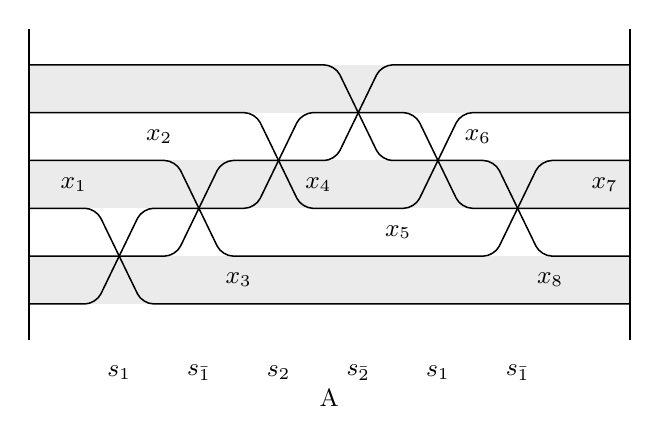
\begin{tikzpicture}[scale=0.92]
\fill[black!8] (0.00,0.00) rectangle (1.25,0.66);
\fill[black!8] (0.00,1.32) rectangle (1.25,1.98);
\fill[black!8] (0.00,2.64) rectangle (1.25,3.30);
\fill[black!8] (1.25,0.00) rectangle (2.35,0.66);
\fill[black!8] (1.25,1.32) rectangle (2.35,1.98);
\fill[black!8] (1.25,2.64) rectangle (2.35,3.30);
\fill[black!8] (2.35,0.00) rectangle (3.45,0.66);
\fill[black!8] (2.35,1.32) rectangle (3.45,1.98);
\fill[black!8] (2.35,2.64) rectangle (3.45,3.30);
\fill[black!8] (3.45,0.00) rectangle (4.55,0.66);
\fill[black!8] (3.45,1.32) rectangle (4.55,1.98);
\fill[black!8] (3.45,2.64) rectangle (4.55,3.30);
\fill[black!8] (4.55,0.00) rectangle (5.65,0.66);
\fill[black!8] (4.55,1.32) rectangle (5.65,1.98);
\fill[black!8] (4.55,2.64) rectangle (5.65,3.30);
\fill[black!8] (5.65,0.00) rectangle (6.75,0.66);
\fill[black!8] (5.65,1.32) rectangle (6.75,1.98);
\fill[black!8] (5.65,2.64) rectangle (6.75,3.30);
\fill[black!8] (6.75,0.00) rectangle (8.30,0.66);
\fill[black!8] (6.75,1.32) rectangle (8.30,1.98);
\fill[black!8] (6.75,2.64) rectangle (8.30,3.30);
\draw[line width=0.55pt, rounded corners=4pt] (0.00,0.00) -- (0.93,0.00) -- (1.25,0.66) -- (1.57,1.32) -- (3.13,1.32) -- (3.45,1.98) -- (3.77,2.64) -- (5.33,2.64) -- (5.65,1.98) -- (5.97,1.32) -- (8.30,1.32);
\draw[line width=0.55pt, rounded corners=4pt] (0.00,0.66) -- (2.03,0.66) -- (2.35,1.32) -- (2.67,1.98) -- (4.23,1.98) -- (4.55,2.64) -- (4.87,3.30) -- (8.30,3.30);
\draw[line width=0.55pt, rounded corners=4pt] (0.00,1.32) -- (0.93,1.32) -- (1.25,0.66) -- (1.57,0.00) -- (8.30,0.00);
\draw[line width=0.55pt, rounded corners=4pt] (0.00,1.98) -- (2.03,1.98) -- (2.35,1.32) -- (2.67,0.66) -- (6.43,0.66) -- (6.75,1.32) -- (7.07,1.98) -- (8.30,1.98);
\draw[line width=0.55pt, rounded corners=4pt] (0.00,2.64) -- (3.13,2.64) -- (3.45,1.98) -- (3.77,1.32) -- (5.33,1.32) -- (5.65,1.98) -- (5.97,2.64) -- (8.30,2.64);
\draw[line width=0.55pt, rounded corners=4pt] (0.00,3.30) -- (4.23,3.30) -- (4.55,2.64) -- (4.87,1.98) -- (6.43,1.98) -- (6.75,1.32) -- (7.07,0.66) -- (8.30,0.66);
\draw[line width=0.7pt] (0.00,-0.50) -- (0.00,3.80);
\draw[line width=0.7pt] (8.30,-0.50) -- (8.30,3.80);
\node[font=\small] at (1.25,-0.95) {$s_1$};
\node[font=\small] at (2.35,-0.95) {$s_{\bar1}$};
\node[font=\small] at (3.45,-0.95) {$s_2$};
\node[font=\small] at (4.55,-0.95) {$s_{\bar2}$};
\node[font=\small] at (5.65,-0.95) {$s_1$};
\node[font=\small] at (6.75,-0.95) {$s_{\bar1}$};
\node[font=\small] at (0.62,1.65) {$x_1$};
\node[font=\small] at (1.80,2.31) {$x_2$};
\node[font=\small] at (2.90,0.33) {$x_3$};
\node[font=\small] at (4.00,1.65) {$x_4$};
\node[font=\small] at (5.10,0.99) {$x_5$};
\node[font=\small] at (6.20,2.31) {$x_6$};
\node[font=\small] at (7.95,1.65) {$x_7$};
\node[font=\small] at (7.20,0.33) {$x_8$};
\node[font=\small] at (4.15,-1.30) {A};
\end{tikzpicture}\par\medskip
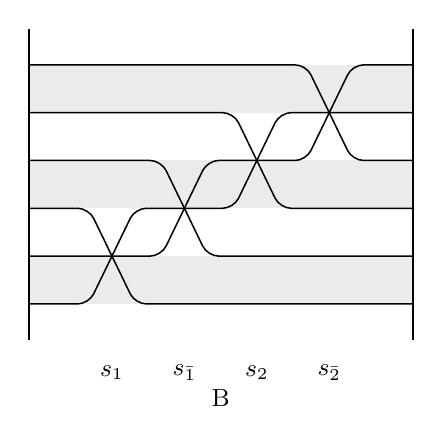
\begin{tikzpicture}[scale=0.92]
\fill[black!8] (0.00,0.00) rectangle (1.15,0.66);
\fill[black!8] (0.00,1.32) rectangle (1.15,1.98);
\fill[black!8] (0.00,2.64) rectangle (1.15,3.30);
\fill[black!8] (1.15,0.00) rectangle (2.15,0.66);
\fill[black!8] (1.15,1.32) rectangle (2.15,1.98);
\fill[black!8] (1.15,2.64) rectangle (2.15,3.30);
\fill[black!8] (2.15,0.00) rectangle (3.15,0.66);
\fill[black!8] (2.15,1.32) rectangle (3.15,1.98);
\fill[black!8] (2.15,2.64) rectangle (3.15,3.30);
\fill[black!8] (3.15,0.00) rectangle (4.15,0.66);
\fill[black!8] (3.15,1.32) rectangle (4.15,1.98);
\fill[black!8] (3.15,2.64) rectangle (4.15,3.30);
\fill[black!8] (4.15,0.00) rectangle (5.30,0.66);
\fill[black!8] (4.15,1.32) rectangle (5.30,1.98);
\fill[black!8] (4.15,2.64) rectangle (5.30,3.30);
\draw[line width=0.55pt, rounded corners=4pt] (0.00,0.00) -- (0.83,0.00) -- (1.15,0.66) -- (1.47,1.32) -- (2.83,1.32) -- (3.15,1.98) -- (3.47,2.64) -- (5.30,2.64);
\draw[line width=0.55pt, rounded corners=4pt] (0.00,0.66) -- (1.83,0.66) -- (2.15,1.32) -- (2.47,1.98) -- (3.83,1.98) -- (4.15,2.64) -- (4.47,3.30) -- (5.30,3.30);
\draw[line width=0.55pt, rounded corners=4pt] (0.00,1.32) -- (0.83,1.32) -- (1.15,0.66) -- (1.47,0.00) -- (5.30,0.00);
\draw[line width=0.55pt, rounded corners=4pt] (0.00,1.98) -- (1.83,1.98) -- (2.15,1.32) -- (2.47,0.66) -- (5.30,0.66);
\draw[line width=0.55pt, rounded corners=4pt] (0.00,2.64) -- (2.83,2.64) -- (3.15,1.98) -- (3.47,1.32) -- (5.30,1.32);
\draw[line width=0.55pt, rounded corners=4pt] (0.00,3.30) -- (3.83,3.30) -- (4.15,2.64) -- (4.47,1.98) -- (5.30,1.98);
\draw[line width=0.7pt] (0.00,-0.50) -- (0.00,3.80);
\draw[line width=0.7pt] (5.30,-0.50) -- (5.30,3.80);
\node[font=\small] at (1.15,-0.95) {$s_1$};
\node[font=\small] at (2.15,-0.95) {$s_{\bar1}$};
\node[font=\small] at (3.15,-0.95) {$s_2$};
\node[font=\small] at (4.15,-0.95) {$s_{\bar2}$};
\node[font=\small] at (2.65,-1.30) {B};
\end{tikzpicture}
\hspace{1.6em}
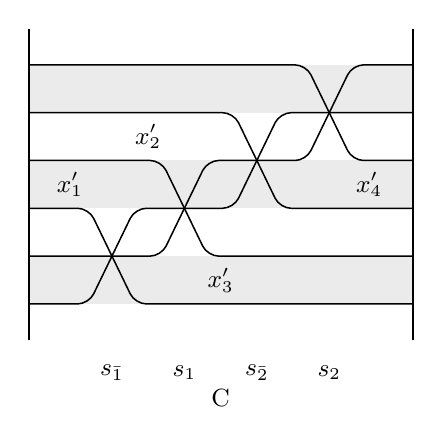
\begin{tikzpicture}[scale=0.92]
\fill[black!8] (0.00,0.00) rectangle (1.15,0.66);
\fill[black!8] (0.00,1.32) rectangle (1.15,1.98);
\fill[black!8] (0.00,2.64) rectangle (1.15,3.30);
\fill[black!8] (1.15,0.00) rectangle (2.15,0.66);
\fill[black!8] (1.15,1.32) rectangle (2.15,1.98);
\fill[black!8] (1.15,2.64) rectangle (2.15,3.30);
\fill[black!8] (2.15,0.00) rectangle (3.15,0.66);
\fill[black!8] (2.15,1.32) rectangle (3.15,1.98);
\fill[black!8] (2.15,2.64) rectangle (3.15,3.30);
\fill[black!8] (3.15,0.00) rectangle (4.15,0.66);
\fill[black!8] (3.15,1.32) rectangle (4.15,1.98);
\fill[black!8] (3.15,2.64) rectangle (4.15,3.30);
\fill[black!8] (4.15,0.00) rectangle (5.30,0.66);
\fill[black!8] (4.15,1.32) rectangle (5.30,1.98);
\fill[black!8] (4.15,2.64) rectangle (5.30,3.30);
\draw[line width=0.55pt, rounded corners=4pt] (0.00,0.00) -- (0.83,0.00) -- (1.15,0.66) -- (1.47,1.32) -- (2.83,1.32) -- (3.15,1.98) -- (3.47,2.64) -- (5.30,2.64);
\draw[line width=0.55pt, rounded corners=4pt] (0.00,0.66) -- (1.83,0.66) -- (2.15,1.32) -- (2.47,1.98) -- (3.83,1.98) -- (4.15,2.64) -- (4.47,3.30) -- (5.30,3.30);
\draw[line width=0.55pt, rounded corners=4pt] (0.00,1.32) -- (0.83,1.32) -- (1.15,0.66) -- (1.47,0.00) -- (5.30,0.00);
\draw[line width=0.55pt, rounded corners=4pt] (0.00,1.98) -- (1.83,1.98) -- (2.15,1.32) -- (2.47,0.66) -- (5.30,0.66);
\draw[line width=0.55pt, rounded corners=4pt] (0.00,2.64) -- (2.83,2.64) -- (3.15,1.98) -- (3.47,1.32) -- (5.30,1.32);
\draw[line width=0.55pt, rounded corners=4pt] (0.00,3.30) -- (3.83,3.30) -- (4.15,2.64) -- (4.47,1.98) -- (5.30,1.98);
\draw[line width=0.7pt] (0.00,-0.50) -- (0.00,3.80);
\draw[line width=0.7pt] (5.30,-0.50) -- (5.30,3.80);
\node[font=\small] at (1.15,-0.95) {$s_{\bar1}$};
\node[font=\small] at (2.15,-0.95) {$s_1$};
\node[font=\small] at (3.15,-0.95) {$s_{\bar2}$};
\node[font=\small] at (4.15,-0.95) {$s_2$};
\node[font=\small] at (0.57,1.65) {$x'_1$};
\node[font=\small] at (1.65,2.31) {$x'_2$};
\node[font=\small] at (2.65,0.33) {$x'_3$};
\node[font=\small] at (4.70,1.65) {$x'_4$};
\node[font=\small] at (2.65,-1.30) {C};
\end{tikzpicture}
\caption{Thurston 图。A：词 $\bar112\bar221\bar1$；B：循环词 $\bar112\bar2$；C：循环词 $\bar112\bar2$。（对 B 与 C，左右两边粘合在一起。）}
\label{fig:1.2}
\end{figure}

$G=\operatorname{PGL}(3)$ 的大胞腔由 (1.6) 的一个特例参数化，它对应于 $W\times W$ 的最长元（这里长度 $l=6$）的一个分解。对元素 $\bar112\bar221\bar1$（其 Thurston 图见图 1.2 A），相应的乘积为
\begin{equation}\label{eq:1.10}
\begin{gathered}
(x_1,\dots,x_8)\mapsto H_1(x_1)E_1H_1(x_2)E_{\bar1}H_2(x_3)E_2H_2(x_4)\\
\cdot E_{\bar2}H_1(x_5)E_1H_1(x_6)E_{\bar1}H_1(x_7)H_2(x_8).
\end{gathered}
\tag{1.10}
\end{equation}
\begin{annote}
原文此处的词 $\bar112\bar221\bar1$ 与图 1.2 A 的标签、式 (1.10) 的乘积（对应 $11\bar122\bar211\bar1$）相差一个循环移位。译文两处均照排原文，读者以式 (1.10) 的乘积为准。
\end{annote}

坐标 $x_1,\dots,x_8$ 分别联系于线段 $]1]$、$[1\bar1]$、$]1\bar12]$、$[2\bar2]$、$[2\bar11\bar1[$、$[11\bar1]$、$[\bar1[$、$[2\bar11\bar1[$。

对 $G/\operatorname{Ad}H$ 中维数为 $l=2\operatorname{rank}G=4$ 的 Poisson 子流形，对应于最长的循环不可约词 $\bar112\bar22$（其 Thurston 图见图 1.2 B），参数化 (1.6) 给出
\begin{equation}\label{eq:1.11}
\begin{aligned}
(x_1,x_2,x_3,x_4)\mapsto{}&H_1(x_1)E_1H_1(x_2)E_{\bar1}H_1(x_3)E_2H_1(x_4)E_{\bar2}\\
={}&\begin{pmatrix}1&1&0\\0&1&0\\0&0&1\end{pmatrix}
\begin{pmatrix}x_1&0&0\\0&1&0\\0&0&1\end{pmatrix}
\begin{pmatrix}1&0&0\\1&1&0\\0&0&1\end{pmatrix}
\begin{pmatrix}x_2&0&0\\0&1&0\\0&0&1\end{pmatrix}\\
&{}\times
\begin{pmatrix}1&0&0\\0&1&1\\0&0&1\end{pmatrix}
\begin{pmatrix}x_3&0&0\\0&x_3&0\\0&0&1\end{pmatrix}
\begin{pmatrix}1&0&0\\0&1&0\\0&1&1\end{pmatrix}
\begin{pmatrix}x_4&0&0\\0&x_4&0\\0&0&1\end{pmatrix}\\
={}&\begin{pmatrix}
x_1x_2x_3x_4+x_2x_3x_4&x_3x_4+x_4&1\\
x_2x_3x_4&x_3x_4+x_4&1\\
0&x_4&1
\end{pmatrix},
\end{aligned}
\tag{1.11}
\end{equation}
其中最后一个矩阵应理解为 $\operatorname{PGL}(3)$ 的元素，即模去常数倍。

词 $\bar112\bar22$ 的参数化（相应的 Thurston 图见图 1.2 C）由下式给出：
\[
\begin{aligned}
(x'_1,x'_2,x'_3,x'_4)\mapsto{}&H_1(x'_1)E_{\bar1}H_1(x'_2)E_1H_1(x'_3)E_{\bar2}H_1(x'_4)E_2\\
={}&\begin{pmatrix}
x'_1x'_2x'_3x'_4&x'_1x'_3x'_4&x'_1x'_3\\
x'_1x'_2x'_3x'_4&x'_1x'_3x'_4+x'_3x'_4&x'_1x'_3+x'_3\\
0&x'_3x'_4&x'_3+1
\end{pmatrix},
\end{aligned}
\]
其中坐标 $x'_1,x'_2,x'_3,x'_4$ 与坐标 $x_1,x_2,x_3,x_4$ 由关于变量 $x_2$ 与 $x_4$ 的变异相联系：
\[
(x'_1,x'_2,x'_3,x'_4)=\Bigl(x_1(1+x_2)(1+1/x_4)^{-1},\ 1/x_2,\ x_3(1+1/x_2)^{-1}(1+x_4),\ 1/x_4\Bigr).
\]

$\operatorname{PGL}(3)$ 中对应于辛叶的 Poisson 结构可以用交换图来描述，见附录 1.11。对 $\operatorname{PGL}(3)$ 的大胞腔，对应于词 $u=\bar112\bar221\bar1\in W\times W$，相应的图见图 1.21；而对 $G/\operatorname{Ad}H$ 中对应于 $u=\bar112\bar22$ 的 Poisson 子流形，交换图见图 1.22。
